\chapter{Estado del Arte}\label{chapter:state-of-the-art}

En este capítulo, se hará un bogeo de actualidad, tanto por las diferentes aplicaciones que tienen funcionalidades
que podrían acercarse lo que se necesita, como por las posibles plataformas donde desarrollar el software en cuestión,
seleccionando una de ellas para el desarrollo de la aplicación y las librerías que se emplearán para el trabajo con mapas.

\section{Herramientas similares}






\subsection{geojson.io}
\begin{figure}[h]
    \centering
    
\includegraphics[scale=1.5]{Graphics/geojson.io_logo.png}
    \caption{Logo del servicio web geojson.io.}
    \label{fig:figura3}
\end{figure}
Geojson.io \cite*{geojson.io} es un servicio o aplicación web muy útil. Es totalmente gratis y bien conocido en toda la comunidad
de desarrolladores y personas que usan Sistemas de información geográfica hoy en día.
Esta aplicación web se centra en, como ya su
nombre lo deja saber, hacer más fácil la estructuración, visualización y el solapado de archivos que contienen información geográfica vectorial.
Dicha información vectorial es visualizada de manera intuitiva y minimalista en un mapa con muy buen aspecto visual usando el servicio
de mapas de MapBox \cite{mapbox}. El formato de archivo que por excelencia se utiliza para almacenar información geográfica vectorial es \textit{geojson} \cite*{geojsonOfficialPage}.
geojson.io también permite agregar metadatos a los archivos, lo cuál es una característica muy útil para esta información espacial ya almacenada en los archivos.
Como se podrá observar en la siguiente figura(ver figura \ref{fig:figura4}), en un lateral de la pantalla se tiene el mapa y en el otro dos tipos de vistas, la de archivo de texto plano(formato geojson)
y una vista tabular que es bastante útil a la hora de rellenar información sobre las entidades.
\begin{figure}[h]
    \centering
    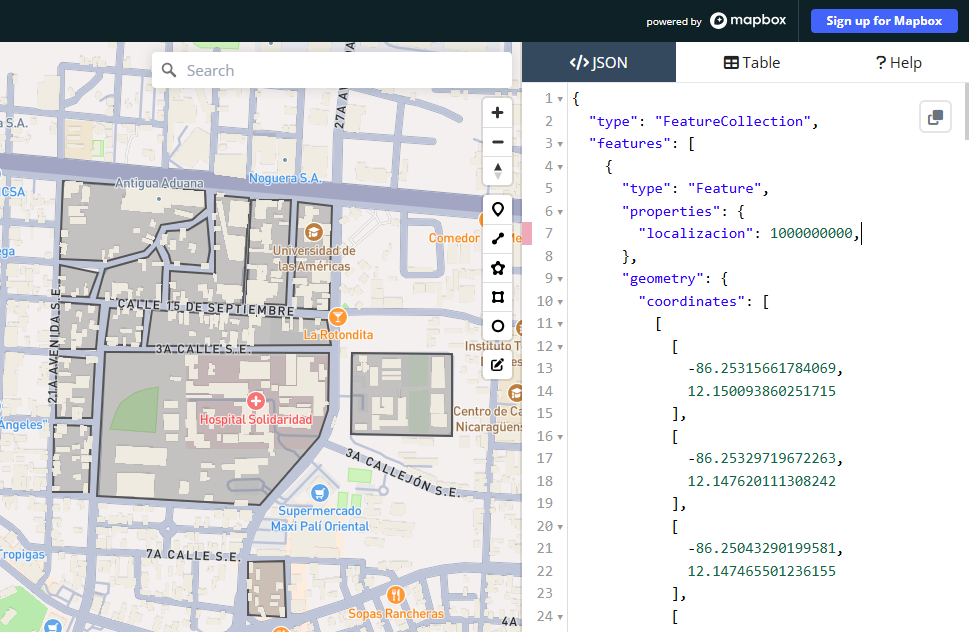
\includegraphics[scale=0.5]{Graphics/geojson.io_description.png}
    \caption{Vista de utilización del servicio geojson.io.}
    \label{fig:figura4}
\end{figure}
Acercándonos al problema de esta tesis, esta página podría resolver varios problemas y puede servir como herramienta para el preprocesado de los datos, como se verá más
adelante en el Capítulo \ref{chapter:proposal}, pero tiene varios aspectos que la alejan de dar solución a lo que necesitamos. Entre los puntos con los que no cumple este servicio
para la solución que se necesita están:
\begin{itemize}
    \item El mapa es cargado con conexión a internet.
    \item No se pueden agregar campos personalizados de tipo fehca o imagen a los metadatos que sirvan luego para almacenar la información que necesitamos de las entidades a encuestar.
    \item No es cómodo acceder a la página desde un dispositivo móvil por el tamaño de la pantalla y, rellenar información ya sea en un archivo de texto plano como lo es geojson o incluso en la vista de tabla puede ser bastante engorroso.
    \item No se puede establecer una relación entre un solo terreno y varias entidades pertenecientes al mismo. Esto es un requerimiento básico del modelo de datos del problema en cuestión.
\end{itemize}






\subsection{Google My Map}
\begin{figure}[h]
    \centering
    
\includegraphics[scale=0.5]{Graphics/google_my_maps_logo.png}
    \caption{Logo del servicio web Google My Maps.}
    \label{fig:figura5}
\end{figure}
Google My Maps \cite{googleMyMaps} es un subdominio del servicio Google Maps, el cuál fue creado como una funcionalidad adicional para permitir a los usuarios
crear sus propios mapas personalizados. Este es un servicio muy parecido a geojson.io, con la diferencia de que aquí es posible agregar campos con imágenes, fechas o de Verdadero/Falso.
También se tiene una vista tabular un poco más intuitiva, aunque aún hay condiciones del problema que no son suplidas con este servicio:
\begin{itemize}
    \item El mapa es cargado con conexión a internet.
    \item No es posible rellenar datos sobre diferentes tuplas relacionadas a un mismo terreno.
    \item Sigue proveyendo un formulario estático, el cuál habría que exportar e importar constantemente para preservar los datos.
\end{itemize}
\begin{figure}[h]
    \centering
    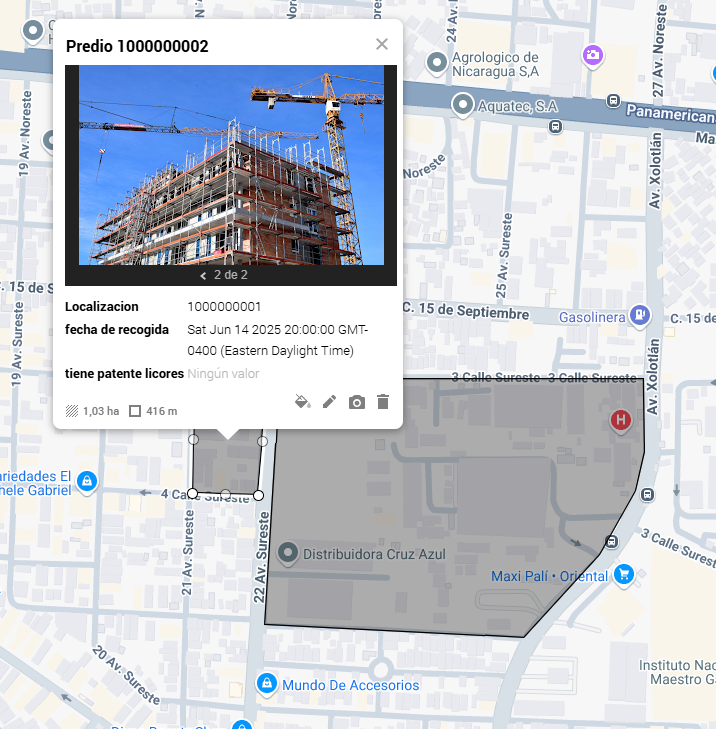
\includegraphics[scale=0.5]{Graphics/google_my_maps_descripcion.png}
    \caption{Vista de utilización del servicio Google My Maps.}
    \label{fig:figura6}
\end{figure}

\pagebreak








\subsection{SW Maps}

\begin{figure}[h]
    \centering
    
\includegraphics[scale=0.5]{Graphics/sw_maps_logo.png}
    \caption{Logo de la aplicación SW Maps.}
    \label{fig:figura7}
\end{figure}
SW Maps es una aplicación móvil de Sistemas de Información Geográfica (SIG) orientada a la recolección de datos espaciales en campo. Desarrollada para plataformas Android, permite capturar, visualizar y editar información geográfica utilizando tanto el GPS interno del dispositivo como receptores GNSS externos, proporcionando así flexibilidad y precisión en el levantamiento de datos.\\\\
Funcionalidades principales:
\begin{itemize}
    \item Creación y edición de entidades espaciales (puntos, líneas y polígonos).
    \item Definición de formularios personalizados para la captura de atributos asociados a cada entidad.
    \item Compatibilidad con diversos formatos de datos geoespaciales: MBTiles, GeoJSON, CSV, entre muchos otros.
    \item Soporte para superposición de capas raster (imágenes georreferenciadas) y capas vectoriales.
    \item Conectividad con servicios de mapas en línea (OpenStreetMap, Google Maps, etc.).
    \item Posibilidad de operar completamente offline, permitiendo el trabajo en áreas sin conectividad.
    \item Exportación de datos recolectados para su posterior análisis en plataformas SIG de escritorio como QGIS \cite*{qgis}.
\end{itemize}

\begin{figure}[h]
    \centering
    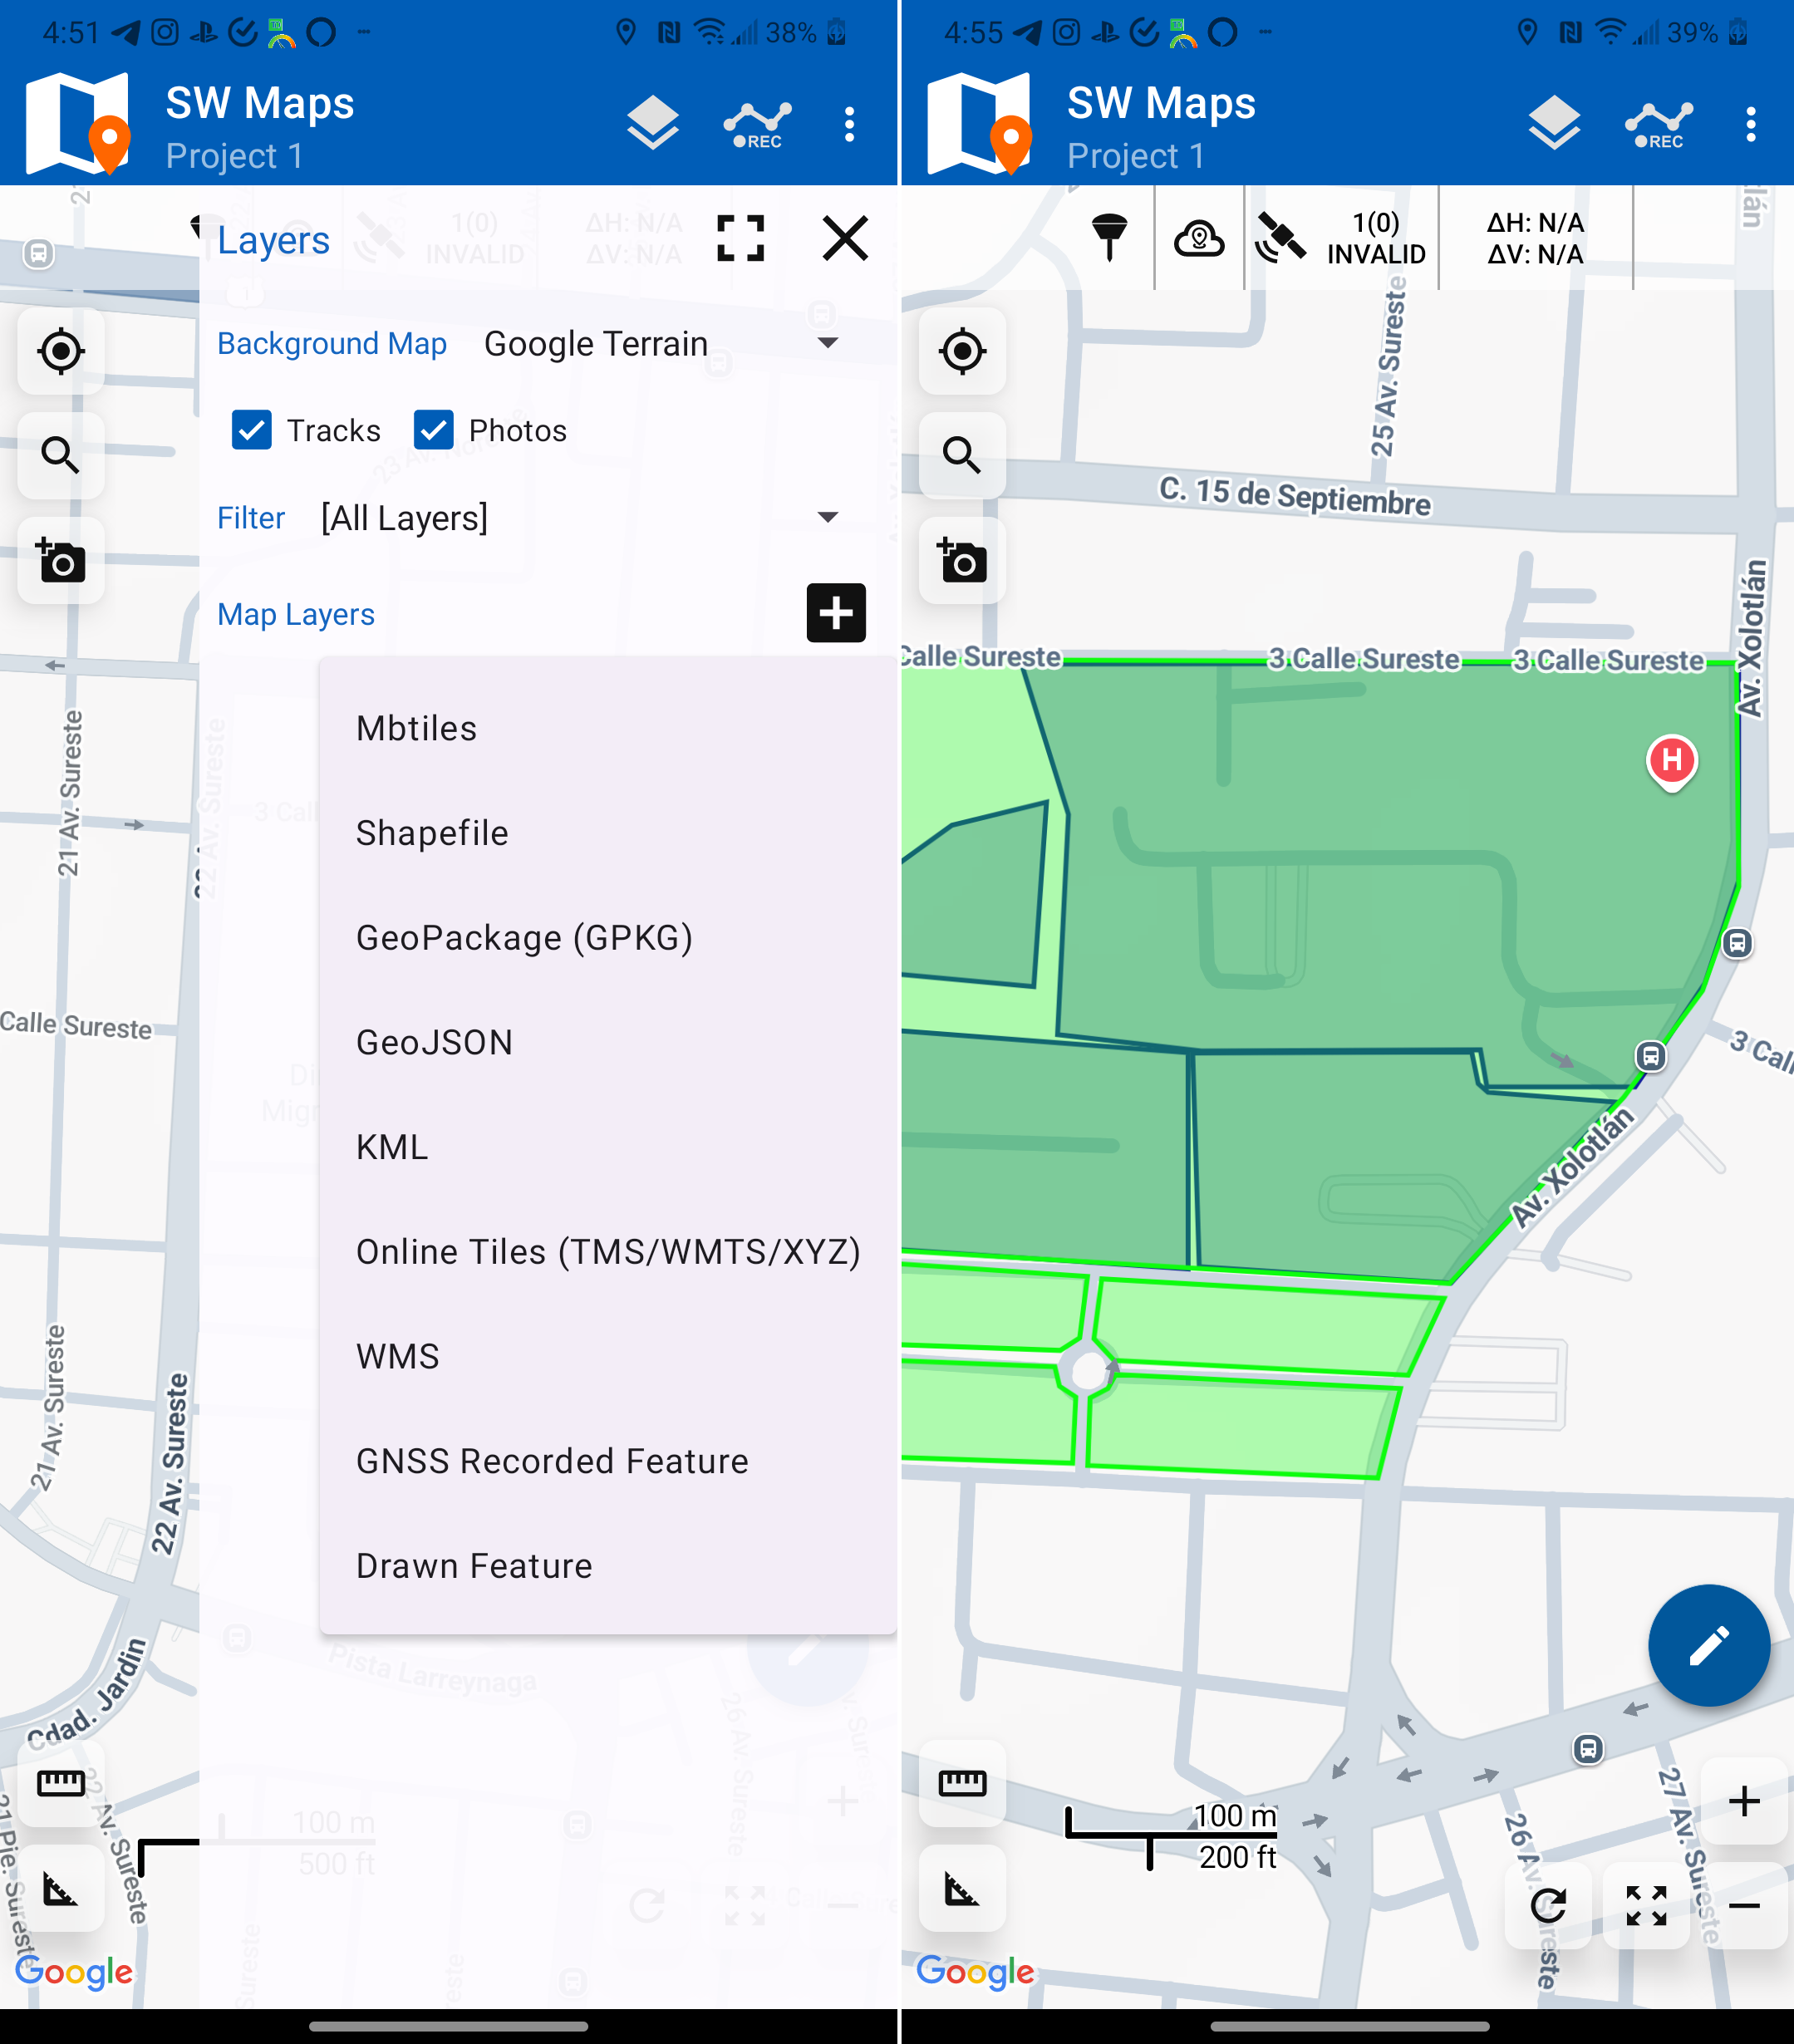
\includegraphics[scale=0.15]{Graphics/sw_maps_importacion.png}
    \caption{Variantes de importación en la aplicación SW Maps.}
    \label{fig:figura8}
\end{figure}

SW Maps es la solución más cercana y conveniente que se encontró en cuanto a solución de los requerimientos del problema. Esta aplicación para Android
tiene la posibilidad de importar y exportar datos geográficos, alimentar estos datos georreferenciadas con metadatos que se rellenan en formularios con una
validación bastante descente, con campos de Verdaero/Falso, imágenes, numéricos e incluso selección simple y selección múltiple.

\begin{figure}[h]
    \centering
    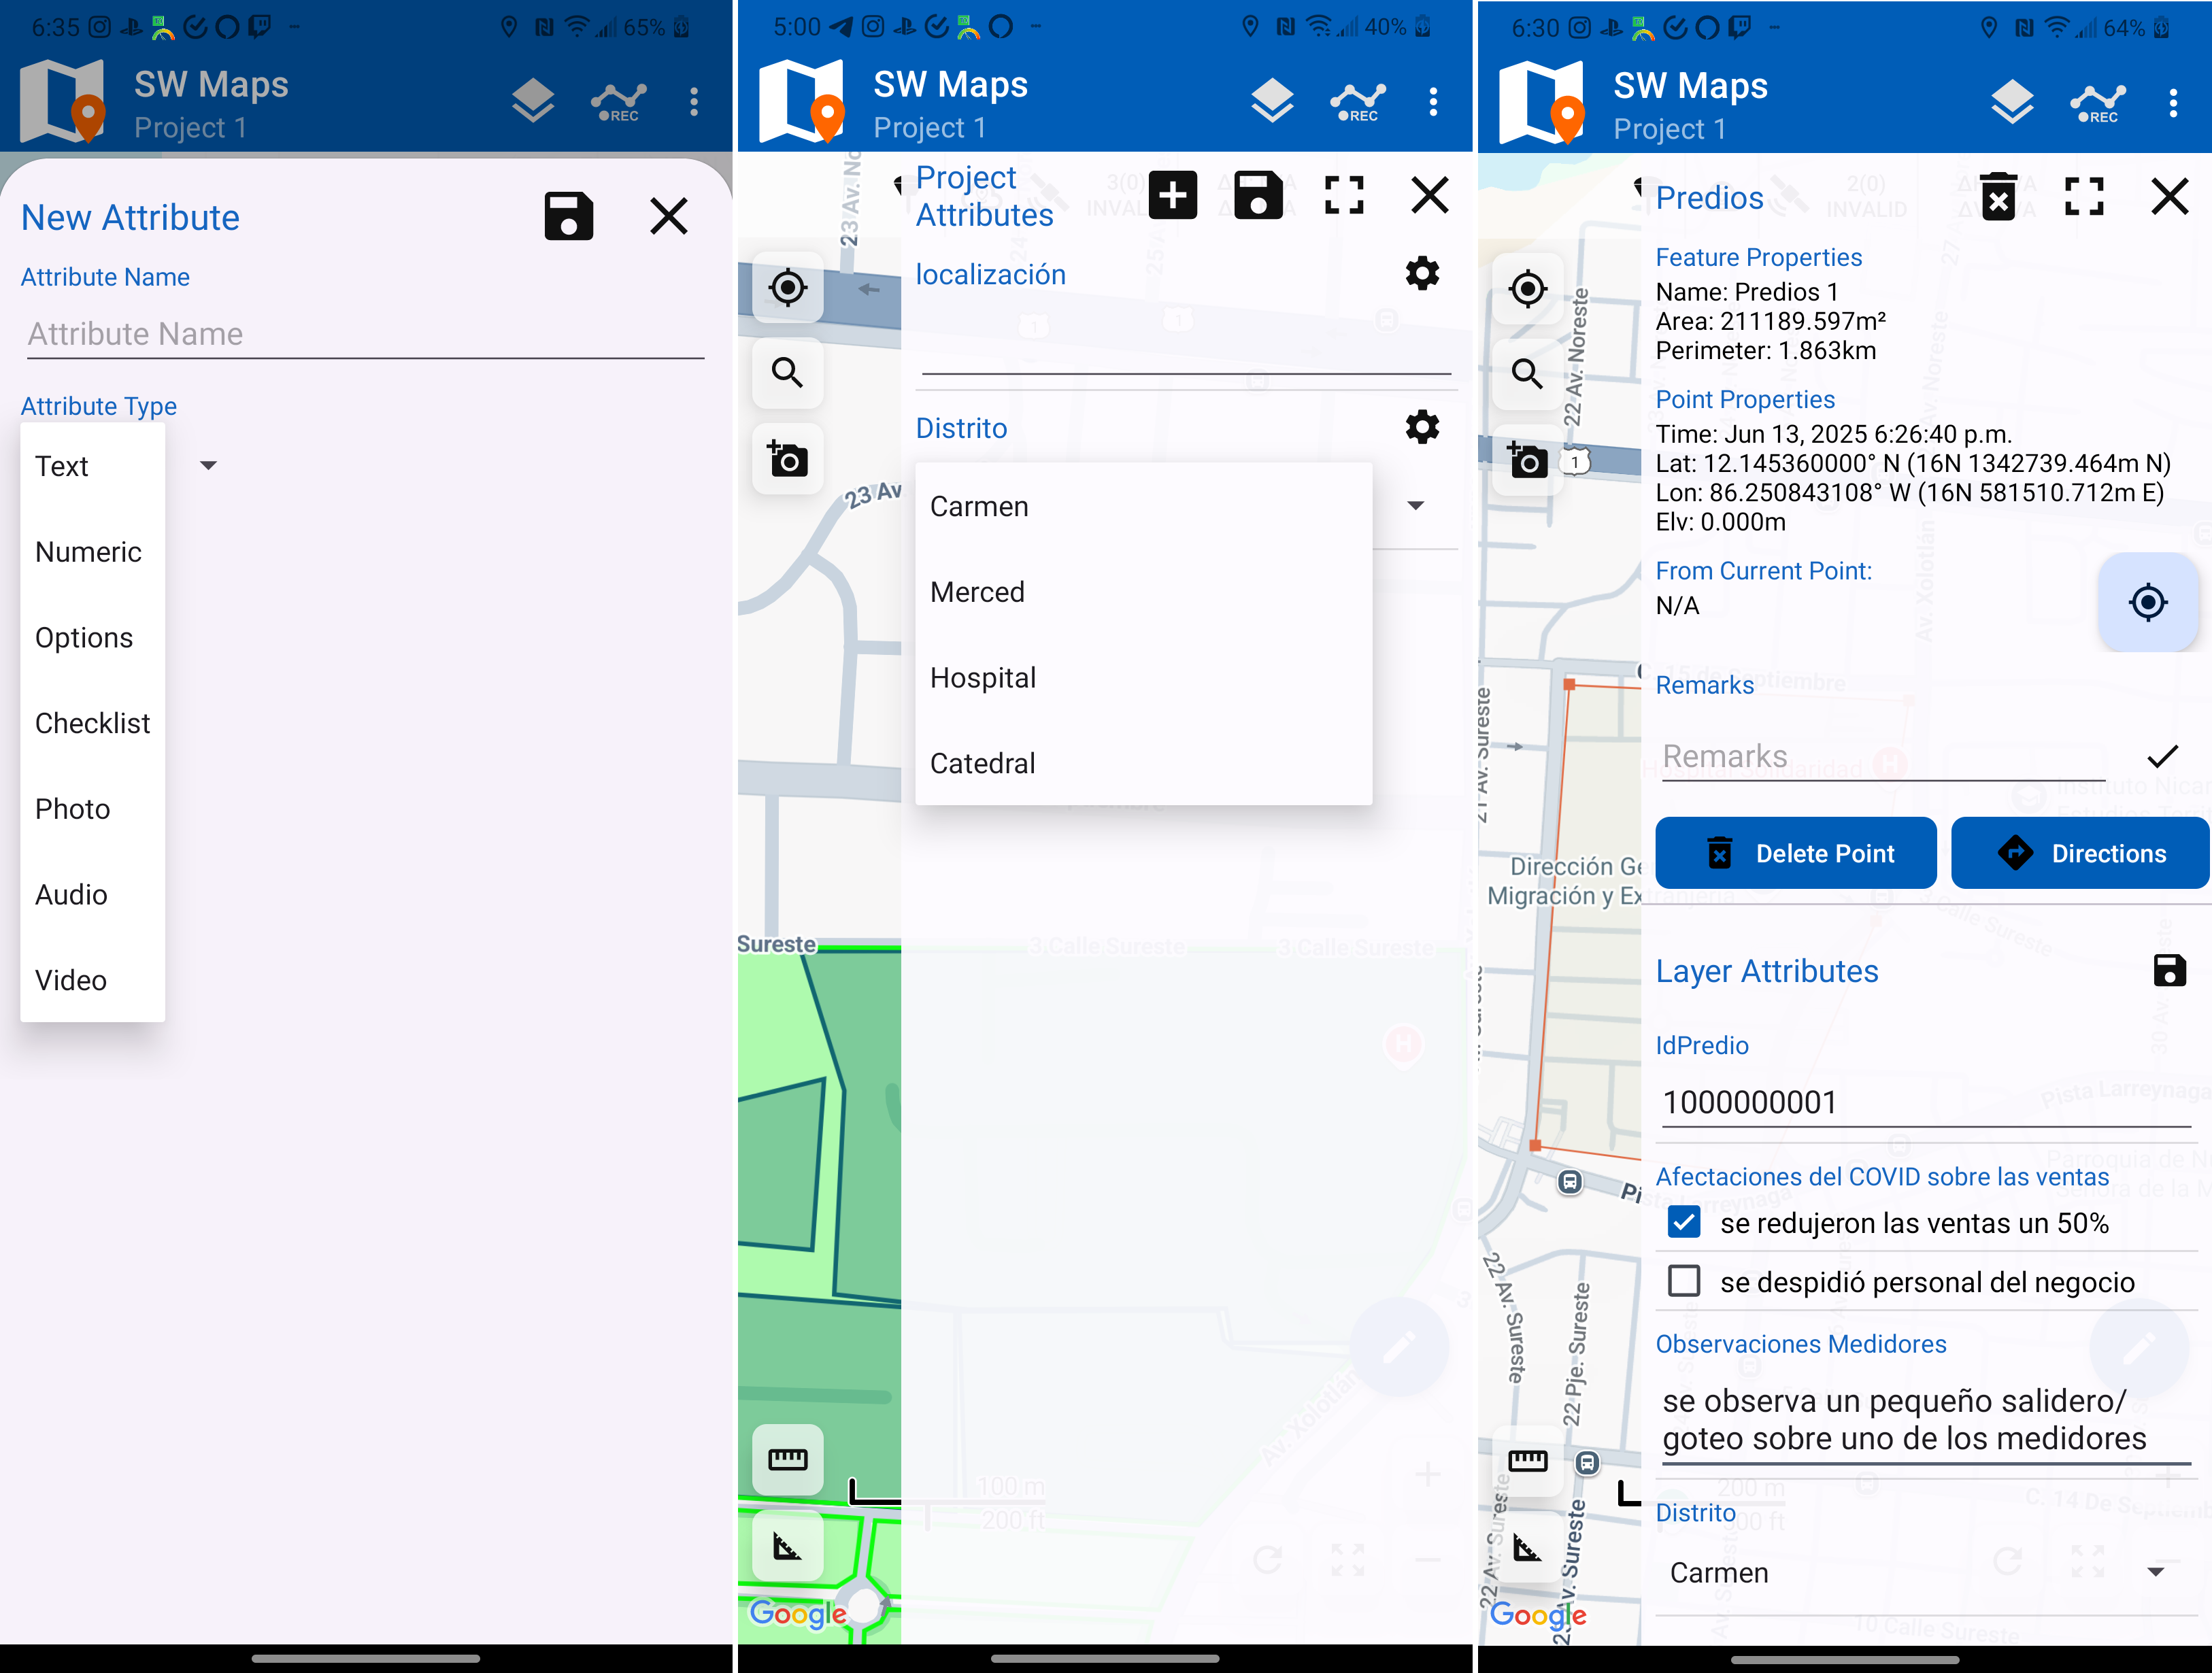
\includegraphics[scale=0.15]{Graphics/sw_maps_campos.png}
    \caption{Variantes de campos de formularios en la aplicación SW Maps.}
    \label{fig:figura9}
\end{figure}

Pero luego de un análisis muy breve se puede observar que esta aplicación tampoco se encuentra ni cerca de ser una posible variante de solución:
\begin{itemize}
    \item Sigue sin ser posible establecer una relación entre un terreno y varias propiedades pertenecientes a la misma área, como lo son las propiedades o locales de diferentes pisos de un mismo edificio. Como ya se dijo, esto es un requisito básico de la naturaleza y los datos del problema.
    \item No se puede hacer ningún tipo de validación extra, que tenga en cuenta por ejemplo, que el número de localización de un predio debe tener específicamente 10 cifras, o que al activar el campo "tiene más patentes" se desbloquea el campo "número de patente 2"
    \item El campo fecha tendría que ser simulado con un campo numérico o de texto, lo cuál no es muy amigable con el usuario y da lugar a que se puedan cometer errores al rellenar este tipo de campos.
    \item No sería posible añadir características intrínsecas de la lógica de negocio del problema, como lo es por ejemplo, que al rellenar los datos de un terreno, este pueda marcarse con otro color para ayudar a los encuestadores a tener una guía de qué terrenos han visitado hasta el momento; lo cuál es una de las razones principales por las que la aplicación solución debe incluir un mapa.
\end{itemize}







\subsection{Conclusiones sobre las diferentes herramientas expuestas}
En esta sección se analizaron aplicaciones con objetivos similares a la aplicación que
se desea desarrollar explicada en el capítulo anterior. Este análisis se realizó con el objetivo
de hacer certera la necesidad de desarrollar una aplicación para Android desde cero. Podemos, dado el análisis anterior, llegar a los siguientes hechos:
\begin{enumerate}
    \item Las herramientas que se exploraron en general no están acorde con las necesidades planteadas por el problema.
          \begin{enumerate}
              \item Muchos de los visores de mapas con que cuentan las aplicaciones analizadas necesitan de
                    internet para mostrar la cartografía. Esto incumple con uno de los requerimientos del cliente.
              \item Muchas de las aplicaciones SIG genéricas están diseñadas con el propósito de rellenar información sobre porciones de terreno, pero en ocasiones se necesita tener no solo información del terreno en general, sino también de los edificios de ese terreno y las propiedades individuales de esos edificios. En este caso es necesario hacer uso de bases de datos relacionales para el correcto almacenamiento de las entidades respresentadas en los datos del problema.
              \item Para una experiencia personalizada de validación de formularios, es preferible y en la mayoría de casos necesario implementar una aplicación desde cero.
          \end{enumerate}
\end{enumerate}
Luego de analizar las aplicaciones anteriores se concluye como necesario el diseño e
implementación de una aplicación que sí cumpla con los requerimientos expuestos en este documento.

\section{Tecnologías de desarrollo de aplicaciones para Android}
\subsection{.NET MAUI}
\begin{figure}[h]
    \centering
    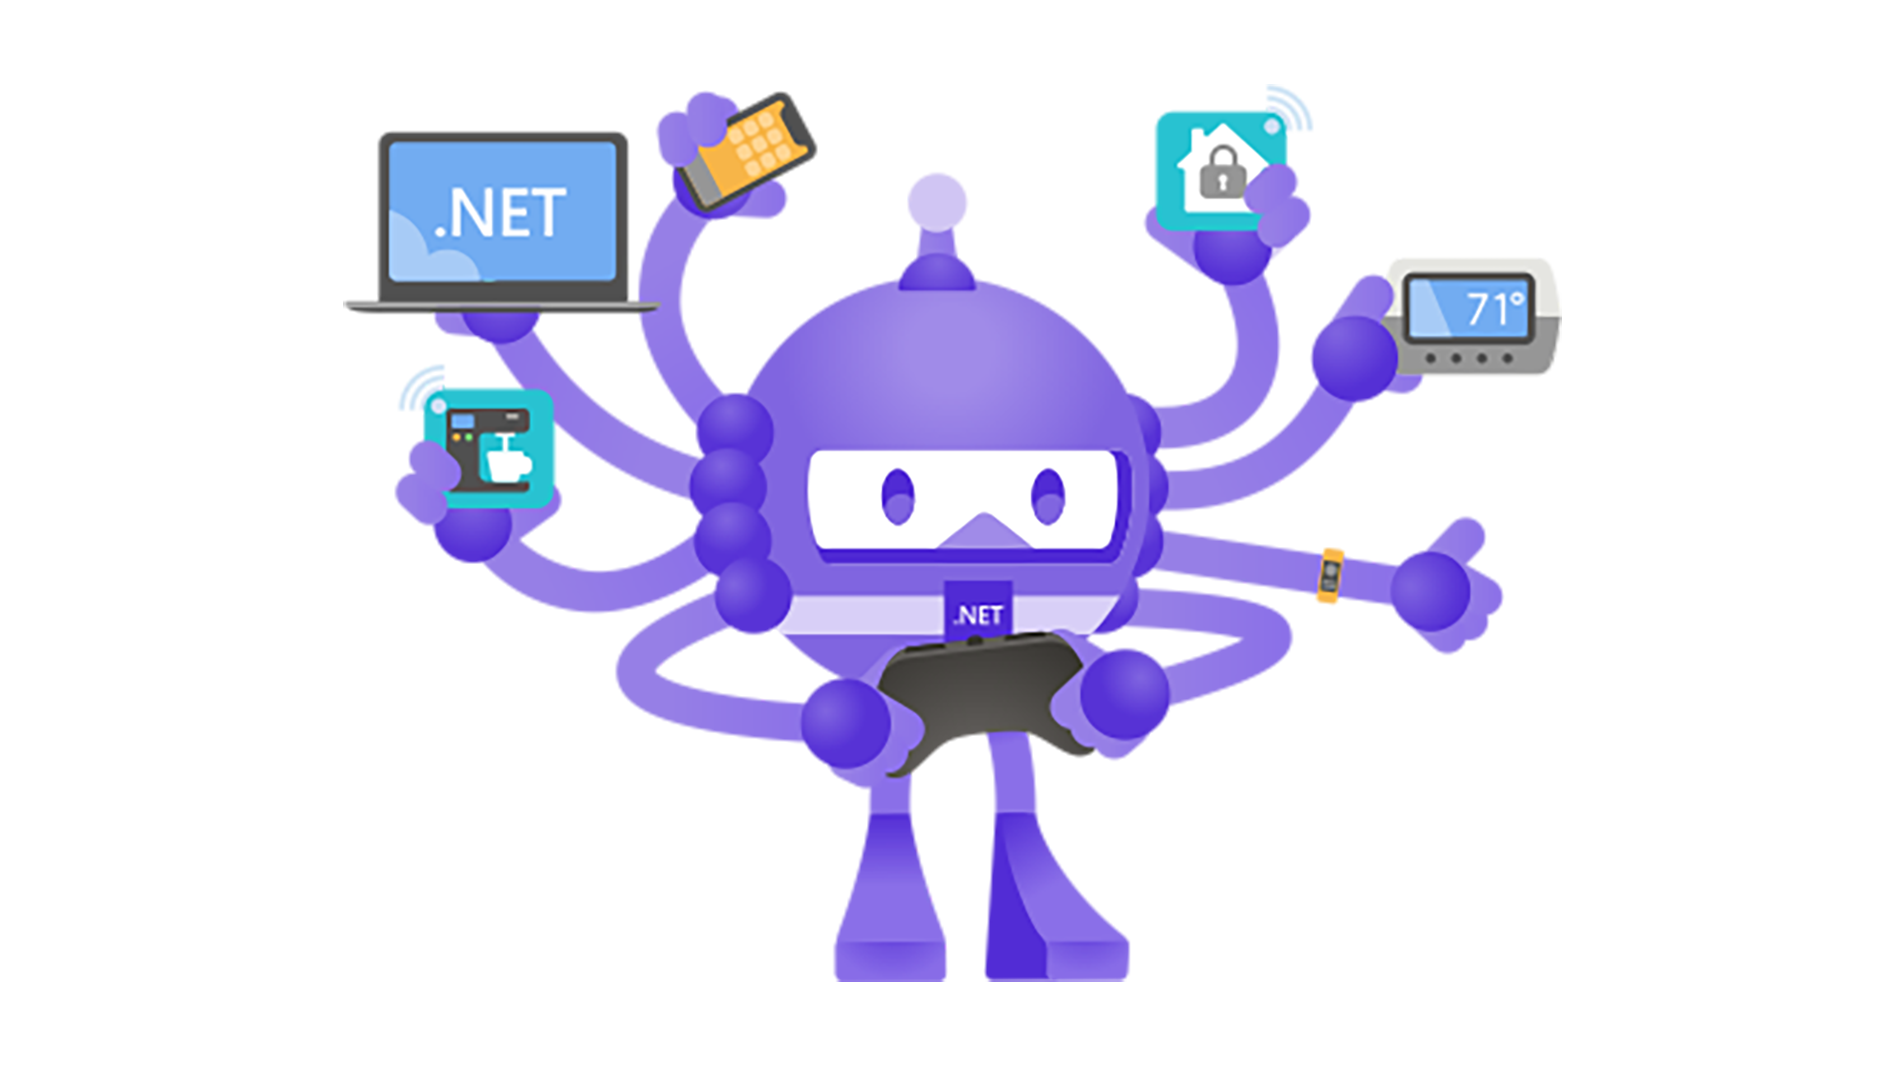
\includegraphics[scale=0.15]{Graphics/MAUI.png}
    \caption{Logo de MAUI.}
    \label{fig:figura10}
\end{figure}
.NET MAUI (Multi-platform App UI) es el framework de desarrollo multiplataforma más reciente de Microsoft, lanzado oficialmente en 2022 como evolución directa de Xamarin.Forms. Forma parte integral del ecosistema .NET 6+.
y permite desarrollar aplicaciones nativas con un único código base para Android, iOS, Windows y macOS
Su arquitectura permite compartir la lógica de negocio, la interfaz de usuario y los recursos entre todas las plataformas, utilizando C\# y XAML como lenguages de programación para el desarrollo.
MAUI unifica los proyectos en una sola estructura de proyecto multiobjetivo, haciendo fácil la administración del código. Compila a código nativo de cada plataforma, accediendo directamente a las APIs nativas sin necesidad de la generación de código intermedio.
Este framework aprovecha la gran comunidad consolidada de desarrolladores .NET y C\# y la comunidad de Xamarin que ha migrado progresivamente hacia acá.
Hay que destacar que Visual Studio ofrece un entorno muy integrado con MAUI a este momento por lo que es una oferta tentadora dada la gran base en el lenguaje C\# proveniente de la carrera.
Destacar el soporte nativo para patrones modernos como MVVM, lo cuál sería una gran tentativa también ya que es la arquitectura escogida para el desarrollo de la aplicación.\\\\
Desventajas:
\begin{itemize}
    \item Aunque hereda parte de la comunidad Xamarin, su base de usuarios aún es más pequeña que Flutter o React Native en el ámbito multiplataforma.
    \item Limitada penetración fuera del ecosistema Microsoft y empresas tradicionales de desarrollo empresarial.
    \item Aunque ha mejorado, la productividad para diseñar UI complejas sigue siendo inferior en comparación con frameworks declarativos como Flutter.
    \item El diseño con XAML puede resultar más verboso y menos intuitivo para nuevos desarrolladores.
    \item Ecosistema de plugins más reducido respecto a Flutter o React Native (aunque en crecimiento).
\end{itemize}

\subsection{React Native}
\begin{figure}[h]
    \centering
    
\includegraphics[scale=0.15]{Graphics/react_native_logo.png}
    \caption{Logo de React Native.}
    \label{fig:figura11}
\end{figure}
React Native es un framework de desarrollo de aplicaciones móviles multiplataforma creado originalmente por Facebook (hoy Meta). Permite desarrollar aplicaciones para Android e iOS utilizando JavaScript o TypeScript, empleando el paradigma declarativo de React para construir interfaces de usuario.
El núcleo de React Native traduce los componentes escritos en JavaScript a componentes nativos equivalentes mediante un sistema de puente (bridge), que permite interactuar con las APIs nativas de cada plataforma. A partir de 2022-2023, React Native está evolucionando hacia un modelo de arquitectura denominado Fabric, que reduce la latencia del bridge y mejora el rendimiento en la interacción entre el código JS y el sistema nativo.
React Native permite un alto grado de reutilización de código, especialmente en la lógica de presentación y en las interfaces de usuario, manteniendo acceso a módulos nativos cuando es necesario para funcionalidades específicas de cada plataforma.
Una de sus ventajas es que tiene una de las comunidades de desarrollo móvil más grandes y activas, una super amplia disponibilidad de documentación, tutoriales, librerías y plugins y además el hecho de ser un ecosistema abierto, respaldado por Meta y miles de contribuyentes en internet.
Posee una gran cantidad de paquetes listos para uso en proyectos reales (navegación, mapas, bases de datos, formularios, etc.) así como una programación clara y minimalista en forma declarativa con React. Otra de las ventajas a considerar de este framework es que dado el largo tiempo en el mercado y el gran uso en el mundo real, se sostiene una compatibilidad constante con nuevas versiones de Android e iOS.\\\\
Desventajas:
\begin{itemize}
    \item A pesar de tener una comunidad de desarrolladores muy numerosa, la calidad de algunas librerías de terceros es desigual; muchas no están siempre bien mantenidas.
    \item Dificultad a veces para encontrar soluciones "oficiales" cuando no existe un paquete bien soportado.
    \item Gestión de dependencias puede complicarse cuando hay múltiples paquetes con actualizaciones incompatibles.
    \item Algunas funciones específicas de hardware o SDKs nativos (por ejemplo, ciertos SDKs de cámaras, sensores avanzados o SDKs comerciales cerrados) pueden requerir escribir módulos nativos (en Java/Kotlin para Android o Swift/Obj-C para iOS).
    \item Cambios frecuentes en versiones mayores (por ejemplo: de la arquitectura clásica al nuevo Fabric) que obligan a adaptarse.
    \item Dependencia del ecosistema Node.js puede generar conflictos de versiones de paquetes.
\end{itemize}


\subsection{Flutter}
\begin{figure}[h]
    \centering
    
\includegraphics[scale=0.15]{Graphics/flutter_logo.png}
    \caption{Logo de Flutter.}
    \label{fig:figura12}
\end{figure}
Flutter es un framework de desarrollo de aplicaciones multiplataforma creado por Google. Permite desarrollar aplicaciones nativas para Android, iOS, Web, Windows, macOS y Linux utilizando un único código base escrito en el lenguaje Dart.
A diferencia de otros frameworks que utilizan un puente (bridge) como se vio anteriormente con React Native, entre el código y las APIs nativas, Flutter renderiza directamente los componentes de interfaz de usuario mediante sus propios motores gráficos (Skia/Impeller), controlando cada píxel de la pantalla. Esto le permite ofrecer una experiencia visual coherente, personalizable y con alto rendimiento en todas las plataformas.
Además de la interfaz de usuario, Flutter permite integrar lógica de negocio, acceso a dispositivos, bases de datos, servicios en la nube y SDKs nativos, mediante canales de plataforma (platform channels) o plugins desarrollados en la propia comunidad.
Hace unos años, desde su primera versión, el desarrollo en esta plataforma ha ido creciendo exponencialmente. Una de las ventajas más fuertes que puede tener Flutter es el respaldado por Google, con fuerte inversión continua en desarrollo y documentación.
Muy buena documentación y Tutoriales en sus plataformas oficiales.
Posee una interfaz de usuario declarativa y reactiva, lo cuál junto con la facilidad de depuración del código lo hacen una gran opción. Posee una gran cantidad de widgets preconstruidos para interfaz de usuario y de paquetes oficiales y de la comunidad disponibles vía pub.dev.\\\\
Desventajas:
\begin{itemize}
    \item Aunque es una de las comunidades que más crece, aún hay menor cantidad de desarrolladores senior comparado con tecnologías como React Native o el ecosistema Android nativo.
    \item Al ser relativamente reciente (2018), algunos escenarios muy específicos aún dependen de la comunidad para ser bien soportados.
    \item La curva inicial de aprendizaje de Dart puede representar un pequeño obstáculo para programadores que provienen de JavaScript o Java.
    \item Para ciertas personalizaciones nativas avanzadas, es necesario desarrollar código nativo en Kotlin/Swift y manejar los Platform Channels.
    \item La dependencia en la calidad de los plugins de terceros puede generar riesgos si algunos quedan desactualizados.
    \item Proyectos muy grandes pueden volverse difíciles de mantener si no se adopta desde el inicio un patrón arquitectónico sólido.
    \item Algunos conceptos (por ejemplo: manejo de estado, inyección de dependencias, modularización) requieren decisiones de arquitectura bien pensadas desde temprano.
\end{itemize}

\subsection{Conclusiones sobre las plataformas de desarrollo expuestas}
Teniendo en cuenta las ventajas y deficiencias en cada uno de los frameworks anteriormente expuestos, hay que decir que las tres plataformas tienen sus ventajas pero Flutter será la escogida
para la implementación de la aplicación dadas todas las ventajas antes expuestas, pero además las necesidades específicas de la implementación que se realizará, dado que se necesita una alta reactividad
en los campos de formularios, ya que se pretende tomar una vertiente moderna y reactiva de la idea de un formulario. Con el potente motor gráfico de Flutter se puede obtener un alto rendimiento en la interfaz.
Este será necesario dada la carga que representa la renderización de mapas, encima con datos geoespaciales personalizados encima, y la función de formularios en la misma zona de ejecución. Flutter es un
framework no tan inexplorado como MAUI y al mismo tiempo viene a resolver deficiencias de React Native, ya que está inspirado en este framework; por lo tanto es una opción razonable e inteligente esta elección.
\section{Librerías para uso de mapas}
\subsection{Librería flutter\_map}
Una implementación en Dart de Leaflet (biblioteca de JavaScript de código abierto
para mapas interactivos aptos para dispositivos móviles) para proporcionar un widget de
mapas para las aplicaciones de Flutter.
El principal atractivo de flutter\_map \cite{flutterMap} en este análisis es la fortaleza y compatibilidad que tiene esta librería con el motor de renderizado
de Flutter, y al unísono, la capacidad de integración con otras librerías que implementan proveedores de teselas, en el caso de la solución a implementar, provenientes de archivos locales
que contengan mapas en el formato que se especificará a continuación.
\subsection{Librería flutter\_map\_mbtiles}
Esta librería proporciona la implementacion de un proovedor de teselas que se configura y carga a partir de archivos locales
en el dispositivo en formato \textbf{.mbtiles}. No solo el proveedor de teselas rasterizadas, sino también capas de polígonos vectoriales y marcadores que son útiles
para la representación de delimitaciones en el mapa, estos a partir polígonos extraídos de archivos en diversos formatos, entre ellos uno de los más populares es \textbf{geojson}.


\subsection{Conclusiones sobre las librerías de mapas}
Se determinó utilizar una combinación de ambas librerías para mostrar tanto el mapa en cuestión como capa base del lienzo, así como también las capas de delimitaciones como
capas extra montadas sobre este mapa base, haciendo uso de la personalización que nos ofrecen estas librerías para hacer marcadores y polígonos informativos que enmarquen
los diferentes predios, manzanas y edificios que se requiran visitar.


\section{Conclusiones del capítulo}
Partiendo de todo lo expuesto en este capítulo de estado del arte resulta importante
resaltar, teniendo en cuenta el estudio de aplicaciones con funcionalidades semejantes
a la deseada, la necesidad de diseñar, desde cero, una aplicación que presente las funcionalidades que se quieren. También consolida la decisión, a partir de los argumentos
expuestos, de tomar como plataforma de desarrollo a Flutter y como gestor de mapas al
paquete flutter\_map cumpliendo con los requerimientos planteados en este documento.
